\documentclass[12pt,a4paper]{article}
\usepackage[utf8]{inputenc}
\usepackage{amsmath}
\usepackage{amsfonts}
\usepackage{amssymb}

\usepackage{placeins}
\usepackage{cmap} % для кодировки шрифтов в pdf
\usepackage[T1]{fontenc}
\usepackage{hhline}
\usepackage[unicode]{hyperref}
\usepackage{multirow}
\usepackage{array}
\usepackage{amsmath}
\usepackage{bm}
\usepackage{textcomp}
\usepackage[russian]{babel}
\usepackage{graphicx} % для вставки картинок
\usepackage{amssymb,amsfonts,amsmath,amsthm} % математические дополнения от АМС
\usepackage{indentfirst} % отделять первую строку раздела абзацным отступом тоже
% Поля
\usepackage{geometry}
\geometry{left=2cm}
\geometry{right=1.5cm}
\geometry{top=2.4cm}
\geometry{bottom=2.cm}

%%%%%%%%%%%%%%%%%%%%%%%%%%%%%%%     

\linespread{1.5} % полуторный интервал
\frenchspacing




\begin{document}
	
	\begin{titlepage}
		
		\begin{center}
			\begin{large}
				Санкт-Петербургский Политехнический университет\\ Петра Великого\\
				Физико-механический институт\\
			\end{large}
			\vspace{0.2cm}
			Высшая школа прикладной математики и вычислительной физики\\
			
		\end{center}
		
		\vspace{3cm}
		\begin{center}
			\textbf{Отчёт\\ по лабораторной работе №1\\ по дисциплине\\ "Компьютерные сети"}
		\end{center}
		
		\vspace{3cm}
		
		\vbox{%
			\hfill%
			\vbox{%
				\hbox{Выполнил студент:}%
				\hbox{\break}
				\hbox{Иванов Андрей Игоревич,}%
				\hbox{группа 5040102$\backslash$20201}%
				\hbox{\break}
				\hbox{\break}
				\hbox{Проверил:}
				\hbox{\break}
				\hbox{к.ф.-м.н., доцент}
				\hbox{Баженов Александр Николаевич}
			}%
		} 
		\vfill
		
		\begin{center}
			Санкт-Петербург, 2024
		\end{center}
	
	\end{titlepage}
	\tableofcontents
	\newpage
	
	\listoffigures
	\newpage
	
	\section{Постановка задачи}
            Задача состоит в реализации системы из двух объектов - отправителя и получателя, которые будут обмениваться сообщениями по каналу связи с помощью протоколов автоматического запроса повторной передачи со скользящего окном: Go-Back-N и Selective Repeat.
            Необходимо проанализировать эффективность работы алгоритмов, рассмотрев следующие зависимости:
            \begin{itemize}
                \item Коэффициент эффективности протокола (отношение числа принятых сообщений к числу отправленных) от ширины окна
                \item Время, затраченное на передачу данных, от ширины окна
                \item Коэффициент эффективности протокола от вероятности потери сообщения
                \item Время, затраченное на передачу данных, от вероятности потери сообщения
            \end{itemize}
        
	\newpage
	
	\section{Теория}
            \subsection{Go-Back-N}
                Go-Back-N — протокол класса ARQ (Automatic Repeat Request), в котором процесс отправки пакета сообщений происходит без подтверждения от получателя. Количество сообщений в пакете определяется размером окна.Фактически, это частный случай общего протокола скользящего окна с размером окна передачи N и размером окна приема 1. Он может передавать N сообщений получаетелю, прежде чем потребуется подтверждение.
    
                Получатель отслеживает порядковый номер следующего сообщения, которое он ожидает получить. Получатель отклоняет сообщение, если оно содержит либо неверный номер, либо если сообщение повторяется или повреждается, иначе переданное сообщение подтверждается. Как только отправитель передал весь пакет, он обнаружит, что все сообщения, начиная с первого потерянного, являются ожидающими, и вернется к порядковому номеру последнего подтверждения, принятого им от получателя, и заполнит его, после чего произойдет повторная передача пакета.
            \subsection{Selective repeat}
                Seletive repeat аналогично является протоколом класса ARQ. В этом случае отправитель передает пакет сообщений без необходимости ждать отдельного подтверждения от получателя, как в случае Go-Back-N. Получатель может выборочно отклонить отдельное сообщение, которое впоследствии будет повторно запрошено. Получатель принимает неупорядоченные сообщения и буферизует их. Отправитель в индивидуальном порядке повторно передает сообшения, время ожидания которых истекло.
	\newpage
	
	\section{Реализация}
		Лабораторная работа выполнена на языке Python 3.10 с помощью загружаемых пакетов Matplotlib, numpy. Исходный код лабораторной работы находится на \href{https://github.com/Drusiand/SPbSTU_Computer_Networks.git}{GitHub репозитории}.
	\newpage
	
	\section{Результаты}  
            \begin{figure}[h!]
                \centering
                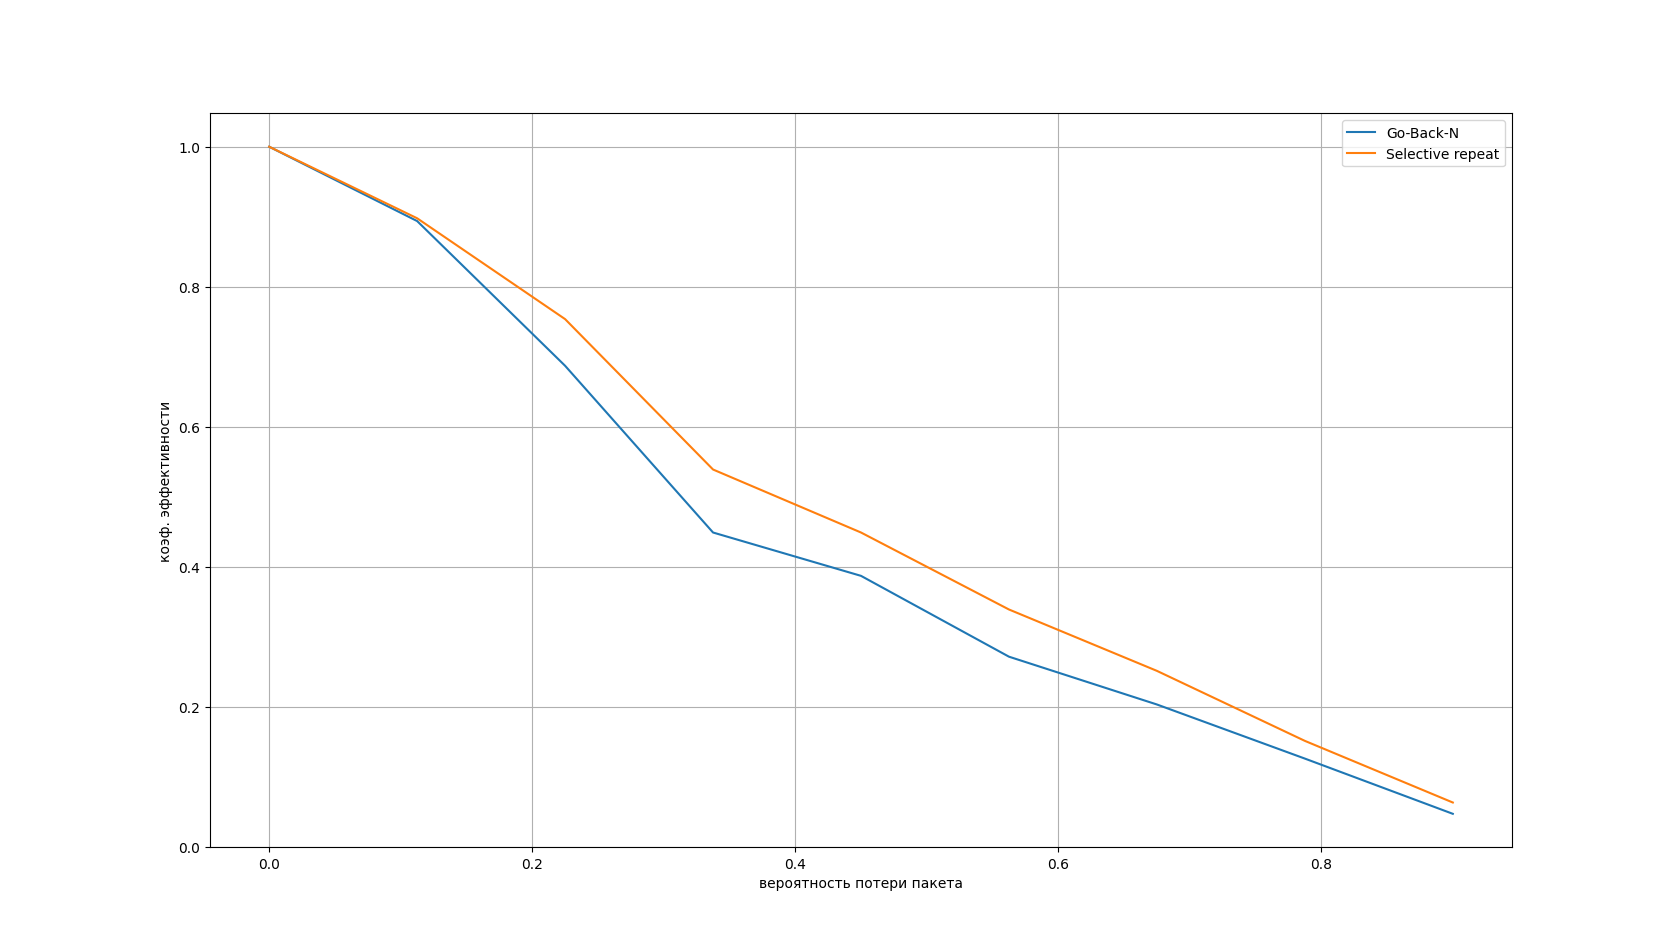
\includegraphics[width=\linewidth]{coeff_prob.png}
                \caption{Зависимость коэффициента эффективности от вероятности потери сообщения}
            \end{figure}
            \FloatBarrier

            \begin{figure}[h!]
                \centering
                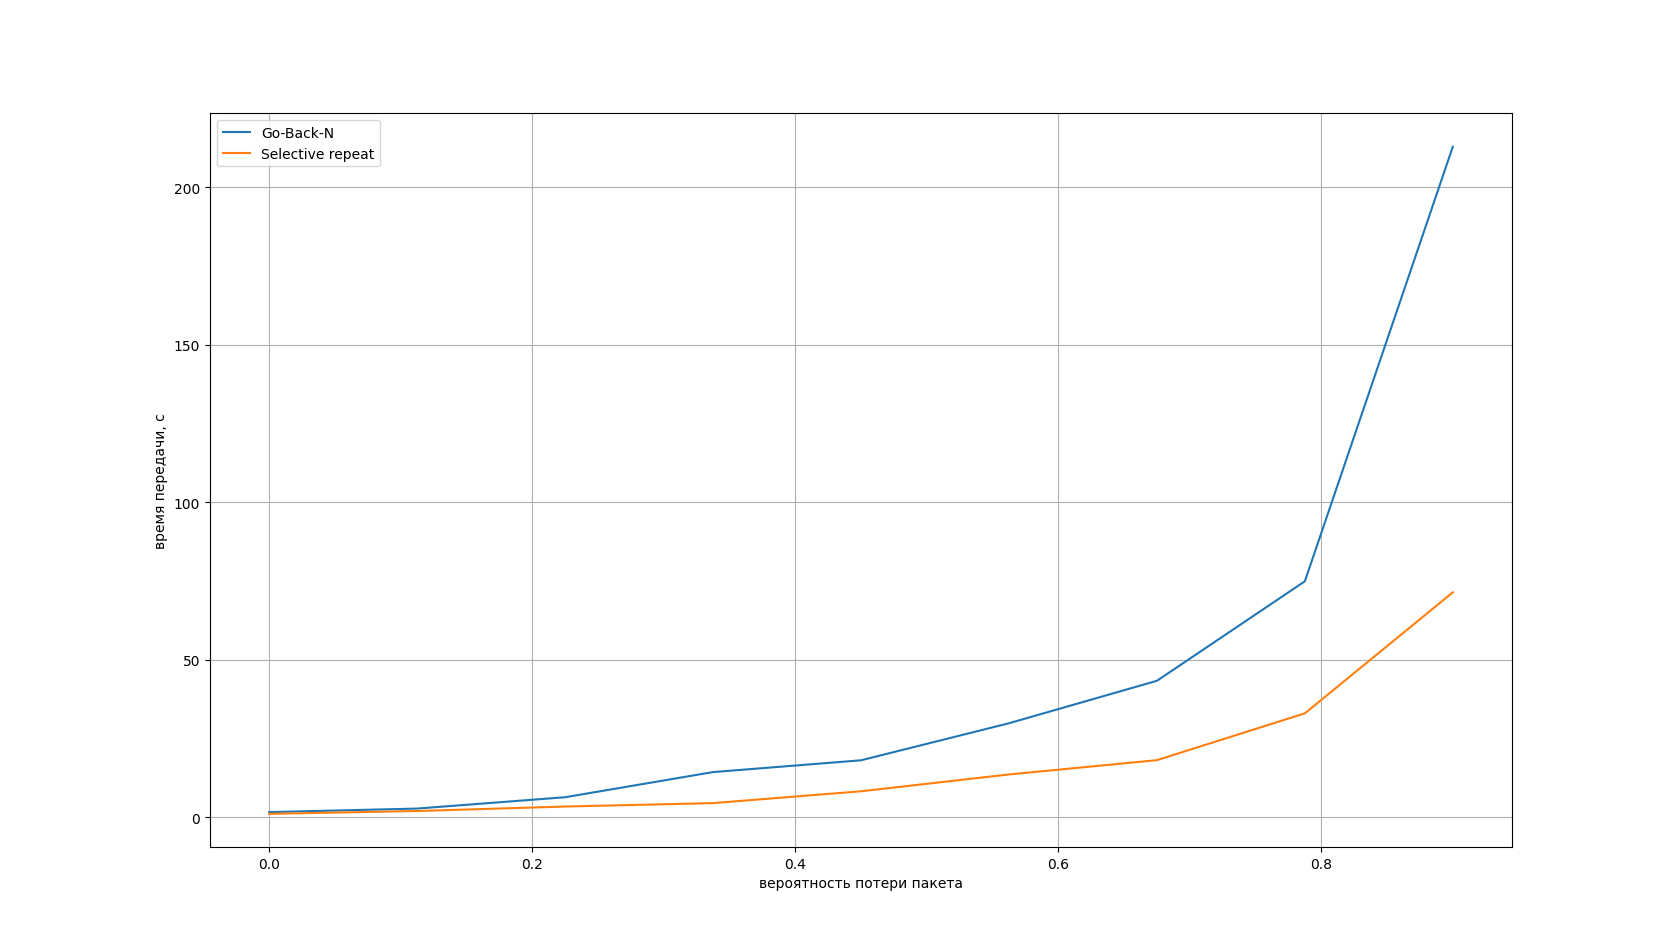
\includegraphics[width=\linewidth]{time_prob.png}
                \caption{Зависимость времени передачи от вероятности потери сообщения}
            \end{figure}
            \FloatBarrier

            \begin{figure}[h!]
                \centering
                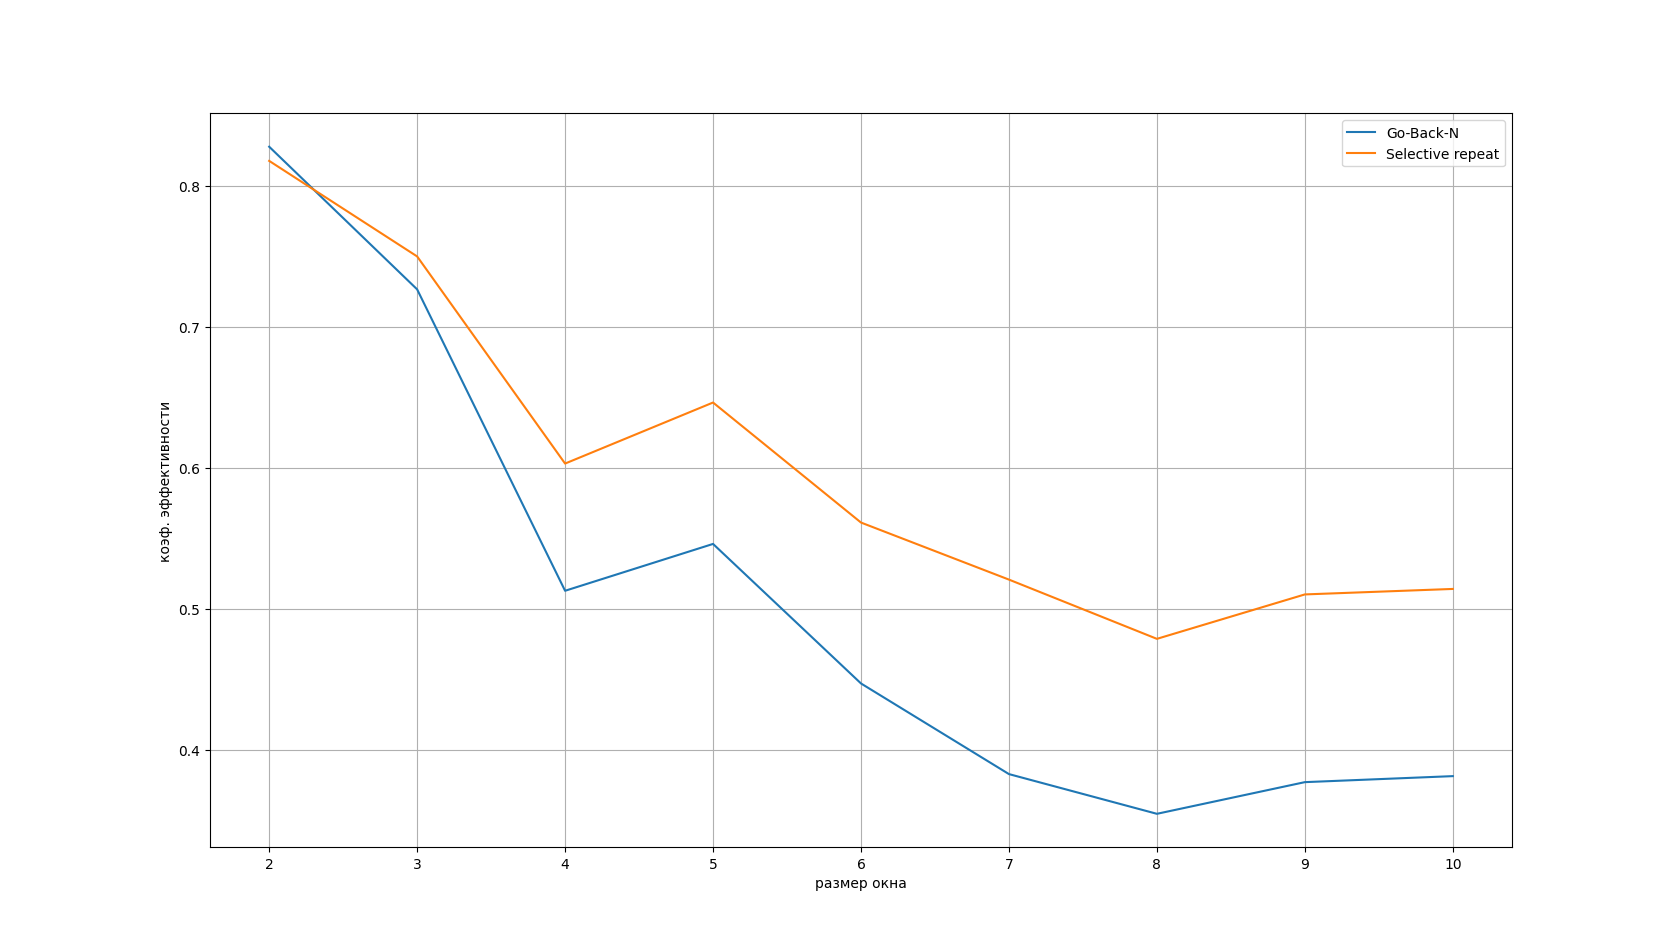
\includegraphics[width=\linewidth]{coeff_window.png}
                \caption{Зависимость коэффициента эффективности от размера окна}
            \end{figure}
            \FloatBarrier

            \begin{figure}[h!]
                \centering
                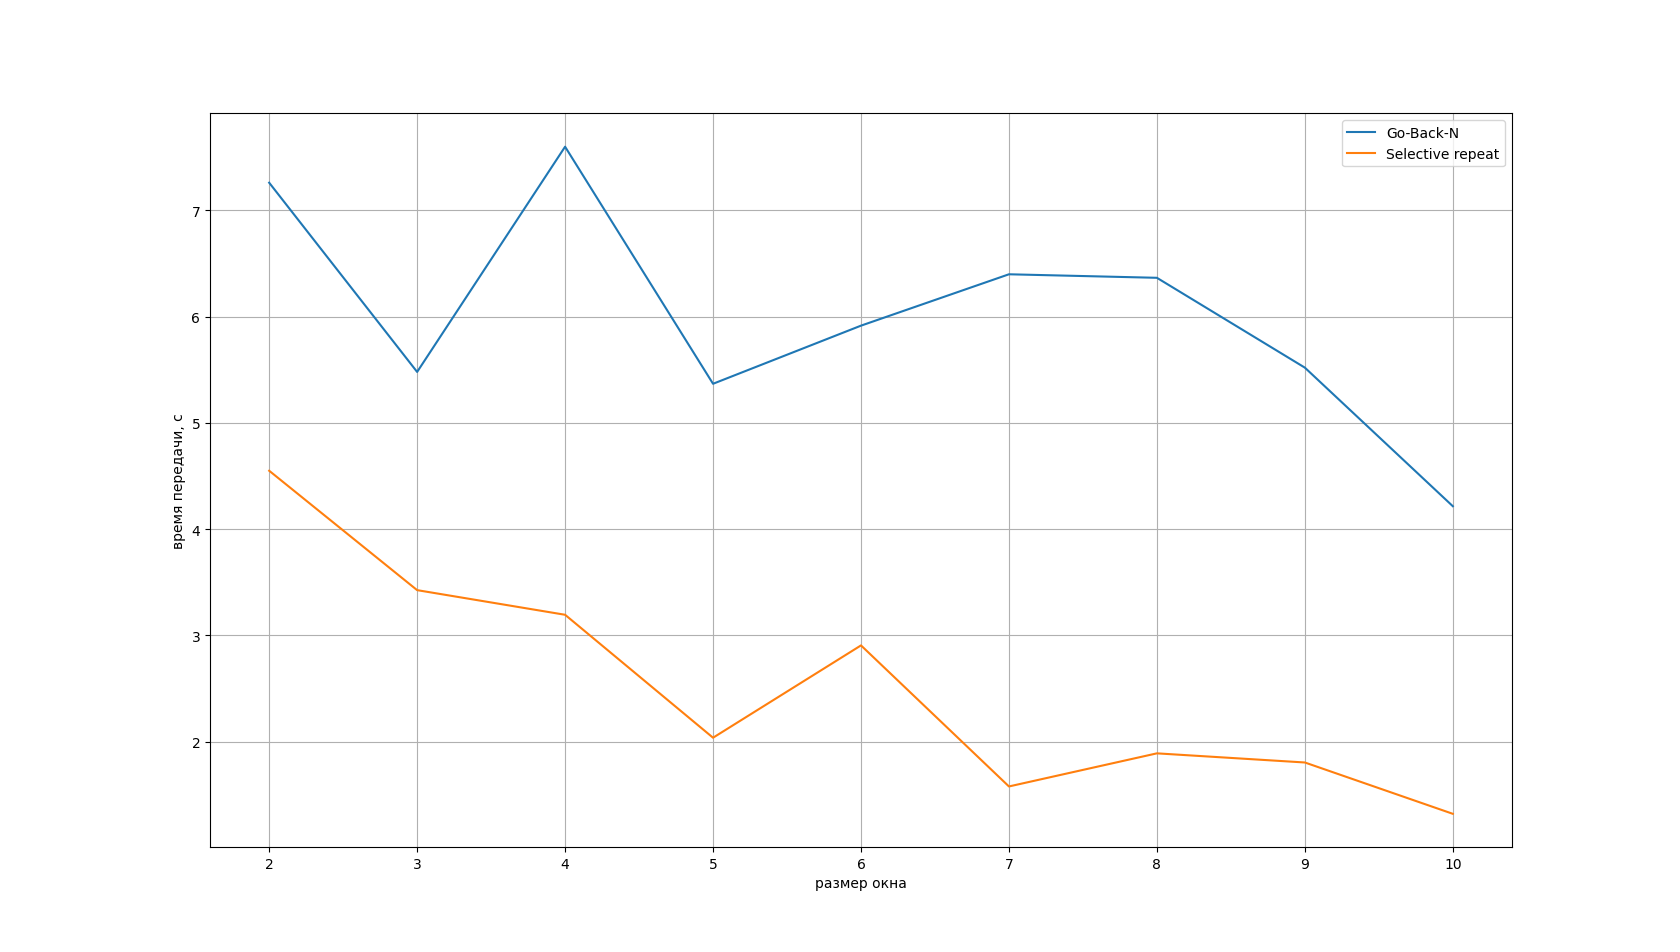
\includegraphics[width=\linewidth]{time_window.png}
                \caption{Зависимость времени передачи от размера окна}
            \end{figure}
            \FloatBarrier
        \clearpage
	\newpage
 
        \section{Вывод}
        Протокол Selective repeat оказался эффективнее Go-Back-N как в плане эффективности передачи данных, так и по времени работы. Go-Back-N показал себя сопоставимым, хоть и уступающим, по эффективности передачи протоколом по сравнению с Selective repeat при равной вероятности потери сообщения, однако для первого наблюдается серьезная задержка при увеличении вероятности.
\end{document}